\lstinputlisting[language=bash,basicstyle=\small]{python_codes/fieldstone_58/keywords}

\noindent \Literature:
\begin{itemize}
\item Compaction creep of sands due to time-dependent grain failure: Effects of chemical environment,
      applied stress, and grain size. Brzesowsky \etal{} (2014) \cite{brhb14}
\item Failure behavior of single sand grains: Theory versus experiment. Brzesowsky \etal{} (2011) \cite{brsp11}
\item Time-independent compaction behavior of quartz sands. Brzesowsky \etal{} (2014) \cite{brsp14}
\item Determination of the tensile strength of rock by a compression test of an 
      irregular test piece. Hiramatsu \etal{} (1966) \cite{hiok66}
\item Micromechanics of sand grain failure and sand compaction. Brzesowsky (1995) \cite{brze95}
\item Contact fatigue in silica sand—Observations and modeling. Wang \& Michalowski (2015) \cite{wami15}
\item Tensile stress concentration and compressive failure in cemented granular material. 
      Wong \& Wu (1995)\cite{wowu95}
\item Micromechanics of pressure-induced grain crushing in porous rocks. Zhang \etal{} (1990) \cite{zhwd90}
\end{itemize}

%----------------------------
\subsubsection*{Experiment 1}

This benchmark is well document in Sadd \cite{sadd14}.
%what follows is from the book itself
Let us investigate the solution to the plane problem shown hereunder of a circular disk 
loaded by equal but opposite concentrated forces along a given diameter. 
This particular problem is of special interest since this geometry is used 
in standard testing of bituminous and other brittle materials such as 
concrete, asphalt, rock, and ceramics. Normally referred to as the Brazilian or indirect tension test, 
the sample and loading geometry create a tension zone along the loaded diameter, 
thus allowing determination of the tensile strength of the specimen material. 
Standard direct tension testing on such brittle materials has led to difficulty 
in establishing a failure region in the sample’s central interior away from 
the gripping locations.

\begin{center}
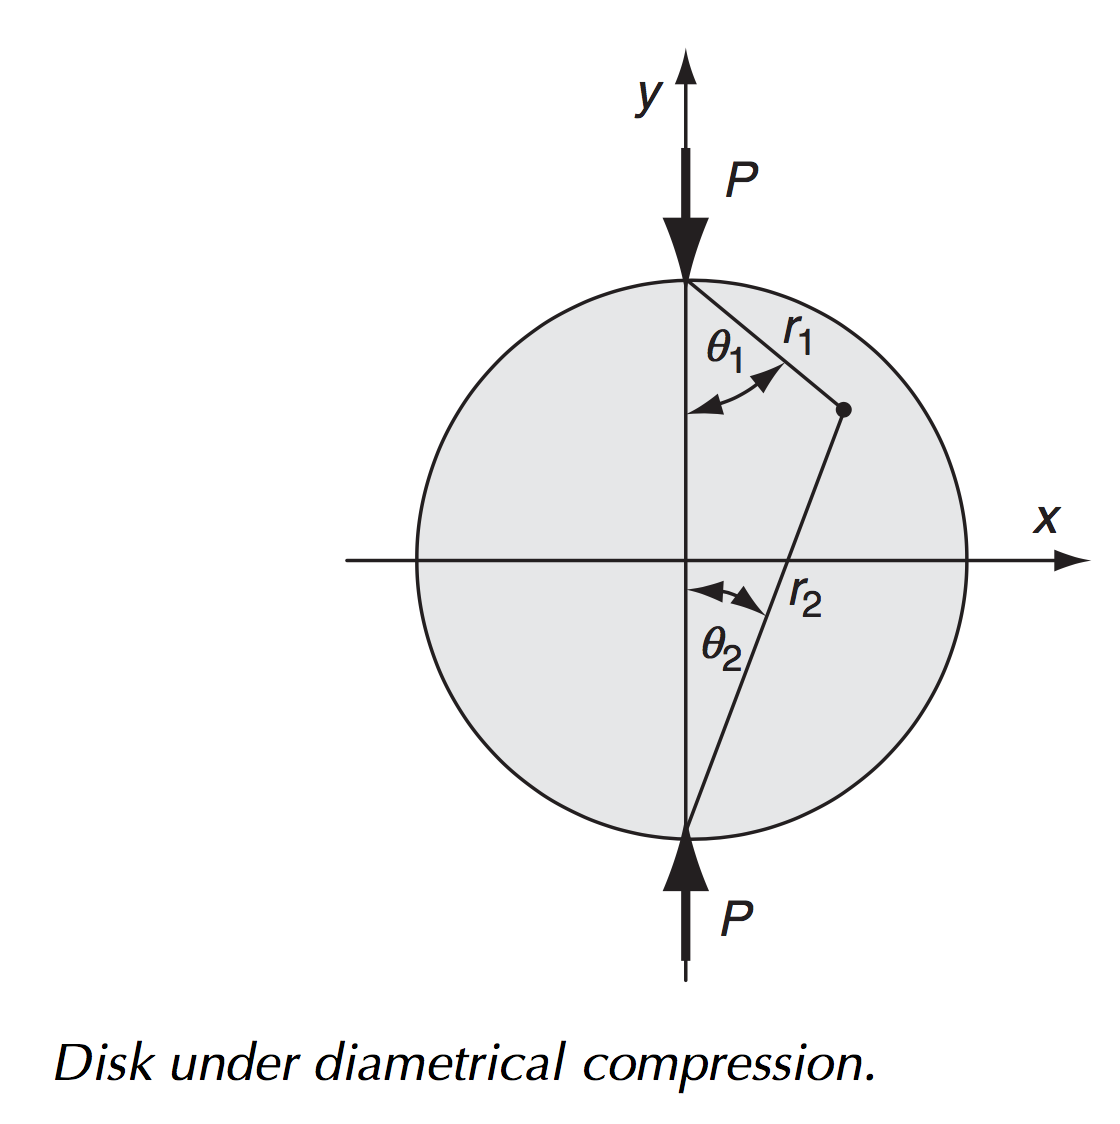
\includegraphics[width=5cm]{python_codes/fieldstone_58/experiment1/setup}\\
{\captionfont Setup of the experiment.}
\end{center}

The mesh is regular and made of concentric layers of triangles. The original algorithm
which was used in \elefant was written by L. van Wiel and is present in the {\tt mesher\_fortran} folder.  
Given the nature of the boundary 
conditions we wish to apply we make sure that two faces are present at the top and bottom 
locations of the disc, which is why the mesh is rotated 90\degree 
after it is generated. \index{contributors}{L. van de Wiel} 

The mesh is composed of {\tt nsection} sections (must be an even number)
as shown hereunder (for {\tt nLayers}=3). 
\begin{center}
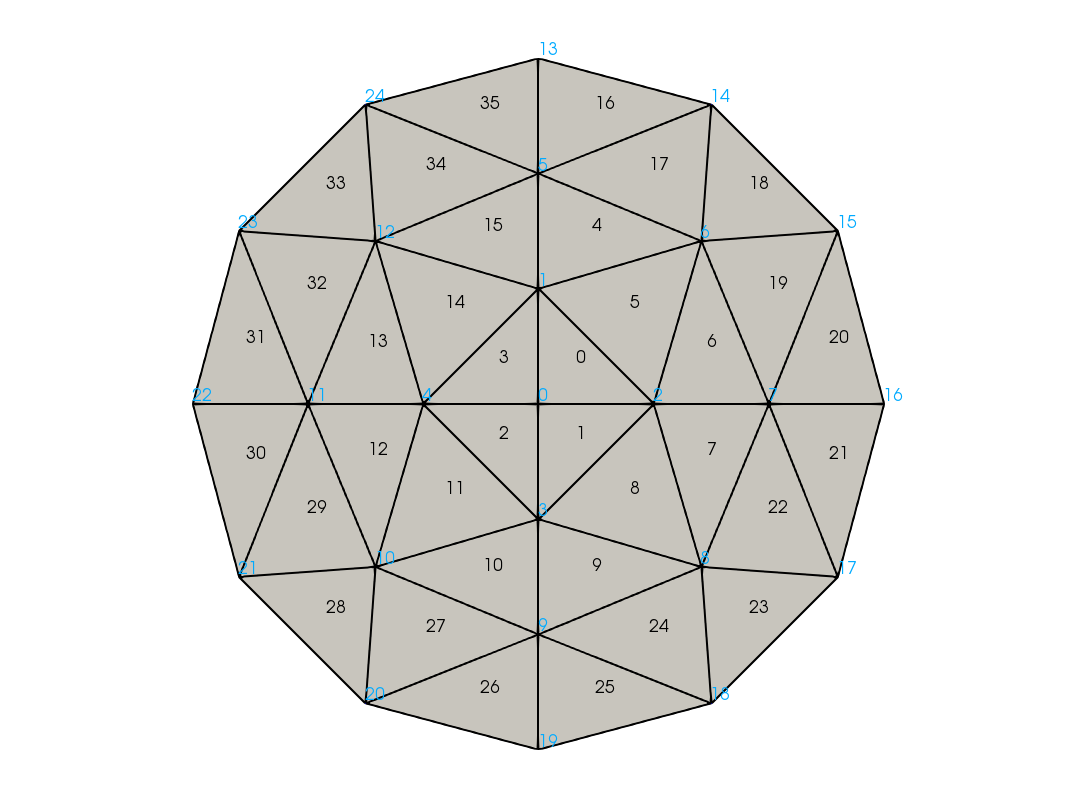
\includegraphics[width=5cm]{python_codes/fieldstone_58/images/mesh4}
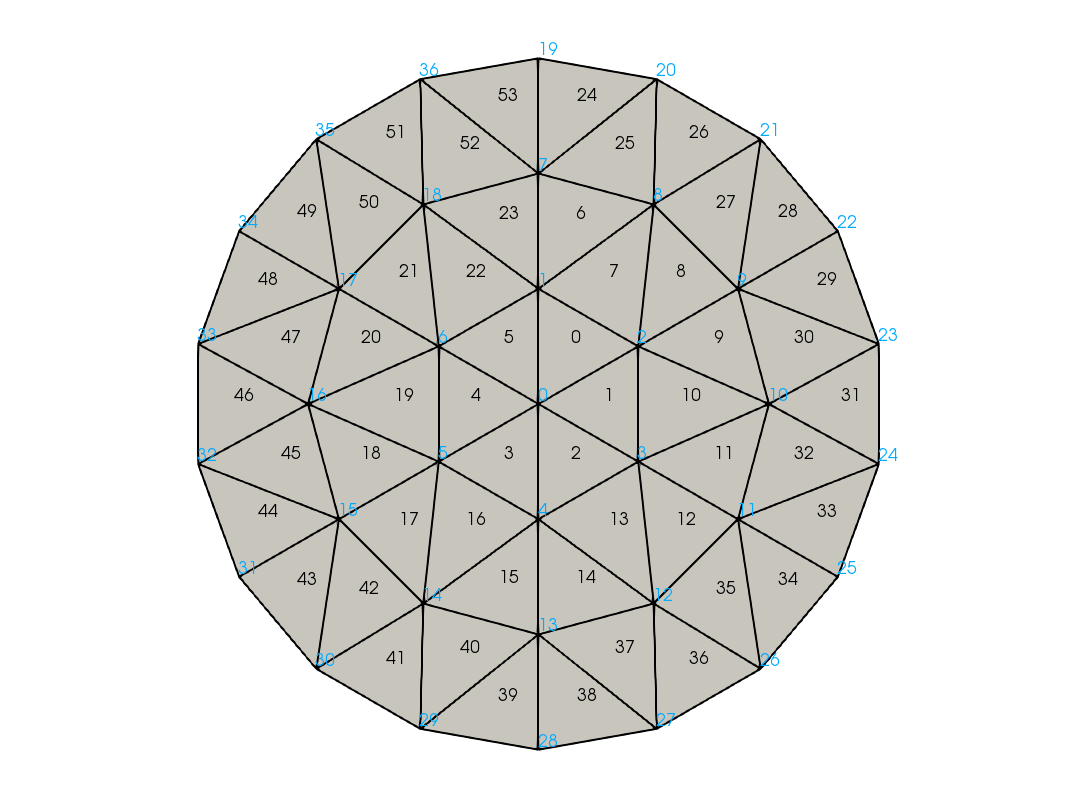
\includegraphics[width=5cm]{python_codes/fieldstone_58/images/mesh6}
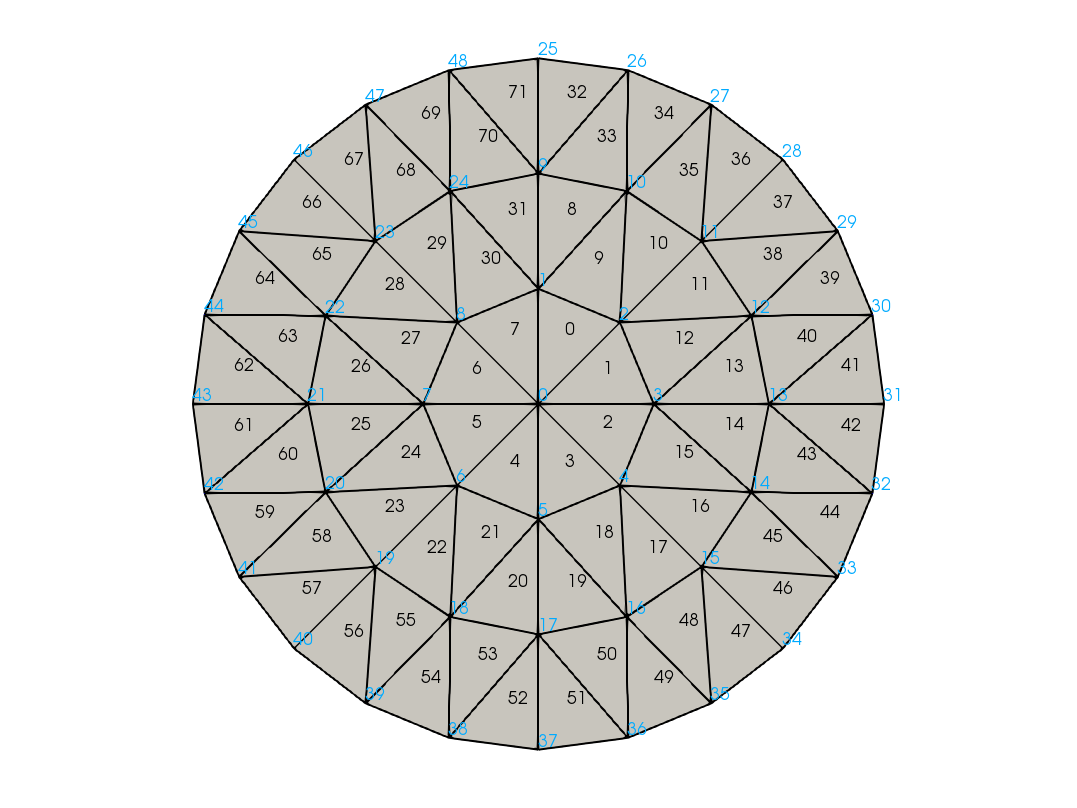
\includegraphics[width=5cm]{python_codes/fieldstone_58/images/mesh8}\\
{\captionfont Mesh composed of 4 sections (left), 6 sections (middle) and 8 sections (right).}
\end{center}

The pressure $P$ prescribed at $y=\pm R$ is actually given by $P \delta({\bm r_\pm})$. 
From \cite{sadd14} (example 8.10, p209), the stress solution is given by:

\begin{eqnarray}
\sigma_{xx}(x,y)&=& -\frac{2P}{\pi}\left[\frac{(R-y)x^2}{r_1^4} + \frac{(R+y)x^2}{r_2^4} -\frac{1}{D} \right] \\
\sigma_{yy}(x,y)&=& -\frac{2P}{\pi}\left[\frac{(R-y)^3}{r_1^4} + \frac{(R+y)^3}{r_2^4} -\frac{1}{D} \right] \\
\sigma_{xy}(x,y)&=&  \frac{2P}{\pi}\left[\frac{(R-y)^2 x}{r_1^4} - \frac{(R+y)^2x}{r_2^4}  \right]
\end{eqnarray}
where 
\[
r_1=\sqrt{x^2 + (R-y)^2}
\quad\quad
r_2=\sqrt{x^2 + (R+y)^2}
\]

The pressure is given by:
\begin{eqnarray}
p(x,y) 
&=& -\frac{1}{2}(\sigma_{xx} + \sigma_{yy}) \nonumber\\
&=& 
 \frac{P}{\pi} \left[ \frac{(R-y)x^2}{r_1^4} + \frac{(R+y)x^2}{r_2^4} -\frac{1}{D} \right] 
+ \frac{P}{\pi} \left[ \frac{(R-y)^3}{r_1^4} + \frac{(R+y)^3}{r_2^4} -\frac{1}{D} \right] \\
&=& 
\frac{P}{\pi} \left[ \frac{(R-y)x^2 + (R-y)^3 }{r_1^4} + \frac{(R+y)x^2 + (R+y)^3}{r_2^4} - \frac{2}{D}\right] 
\end{eqnarray}

On the $x$-axis ($y=0$) these results simplify to give
\begin{eqnarray}
\sigma_{xx}(x,0) &=& \frac{2P}{\pi D} \left( \frac{D^2-4x^2}{D^2+4x^2}  \right)^2 \\
\sigma_{yy}(x,0) &=& -\frac{2P}{\pi D} \left( \frac{4D^4}{(D^2+4x^2)^2} -1 \right) \\
\sigma_{xy}(x,0) &=& 0 \\
p(x,0) 
&=& \frac{P}{\pi} \left[ \frac{(R-y)x^2 + (R-y)^3 }{r_1^4} + \frac{(R+y)x^2 + (R+y)^3  }{r_2^4}  - \frac{2}{D} \right] \\
&=& \frac{P}{\pi} \left[ \frac{Rx^2 + R^3 }{(x^2+R^2)^2} + \frac{Rx^2 + R^3  }{(x^2+R^2)^2}  - \frac{2}{D} \right] \\
&=& \frac{2P}{\pi} \left[ \frac{R(x^2 + R^2 )}{(x^2+R^2)^2} - \frac{1}{D} \right] \\
&=& \frac{2P}{\pi} \left[ \frac{R }{x^2+R^2} - \frac{1}{D} \right] \\
\end{eqnarray}

On the $y$-axis ($x=0$) the stresses are 
\begin{eqnarray}
\sigma_{xx}(0,y) &=& \frac{2P}{\pi D} \\
\sigma_{yy}(0,y) 
&=& -\frac{2P}{\pi} \left( \frac{2}{D-2y} + \frac{2}{D+2y} -\frac{1}{D} \right) \\
&=& -\frac{2P}{\pi} \left( \frac{1}{R-y} + \frac{1}{R+y} -\frac{1}{D} \right) \\
\sigma_{xy} (0,y) &=& 0 \\
p(0,y) 
&=& \frac{P}{\pi} \left[ \frac{(R-y)^3 }{(R-y)^4} + \frac{ (R+y)^3  }{(R+y)^4}  - \frac{2}{D} \right] \\
&=& \frac{P}{\pi} \left[ \frac{1}{R-y} + \frac{ 1 }{R+y}  - \frac{2}{D} \right] 
\end{eqnarray}
In the code the pressure is retrieved after the displacements are computed. 
In 2D, we have (using Eq.~\ref{eq:twoELAST} for the stress tensor):
\begin{eqnarray}
p
&=& -\frac{1}{2}(\sigma_{xx} + \sigma_{yy}) \nonumber\\
&=& -\frac{1}{2} \left[
\lambda (\varepsilon_{xx}+\varepsilon_{yy}) + 2 \mu \varepsilon_{xx} +
\lambda (\varepsilon_{xx}+\varepsilon_{yy}) + 2 \mu \varepsilon_{yy} 
\right] \\
&=& -\frac{1}{2} \left[
2\lambda (\varepsilon_{xx}+\varepsilon_{yy}) + 2 \mu (\varepsilon_{xx} + \varepsilon_{yy} \right]\nn\\
&=& -(\lambda+\mu) (\varepsilon_{xx}+\varepsilon_{yy}) 
\end{eqnarray}

The radius is set to $R=1$, and the disc is centered on the origin. The disc 
is discretised by means of {\sl nlayers} concentric layers of $P_1$ triangles.
I set $\mu=1$ and $\nu=0.25$. 

The boundary conditions are as follows: on the two vertical edges at $y=R$ and $y=-R$ 
the pressure is applied. Furthermore because of the symmetry of the problem, 
and in order to remove the expected nullspaces in the displacement field, 
we fix $u=0$ on the vertical axis and $v=0$ on the horizontal axis.
In the coming plots the number of layers (which needs to be odd) is varied, from 31 to 111.
Note that the displacement is not analytically known but the computed displacement 
nicely converge to a single smooth curve.

\begin{center}
\begin{tabular}{lrrrr}
\hline
{\tt nlayers} & {\tt NV} & {\tt nel} & {\tt Nfem} & $v_{rms}$\\
\hline
\hline
21  &  1387 &  2646 &  2774 & 1.043847e-01\\ 
31  &  2977 &  5766 &  5954 & 1.049944e-01\\
41  &  5167 & 10086 & 10334 & 1.052457e-01\\
51  &  7957 & 15606 & 15914 & 1.053750e-01\\
61  & 11347 & 22326 & 22694 & 1.054509e-01\\
71  & 15337 & 30246 & 30674 & 1.054994e-01\\
81  & 19927 & 39366 & 39854 & 1.055324e-01\\
91  & 25117 & 49686 & 50234 & 1.055560e-01\\
101 & 30907 & 61206 & 61814 & 1.055735e-01\\
111 & 37297 & 73926 & 74594 & 1.055868e-01\\
\hline
\end{tabular}

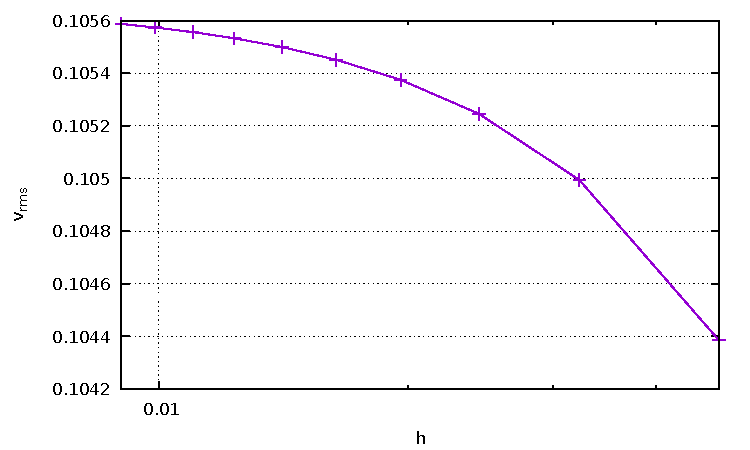
\includegraphics[width=8cm]{python_codes/fieldstone_58/experiment1/vrms}
\end{center}


\newpage
\begin{center}
a)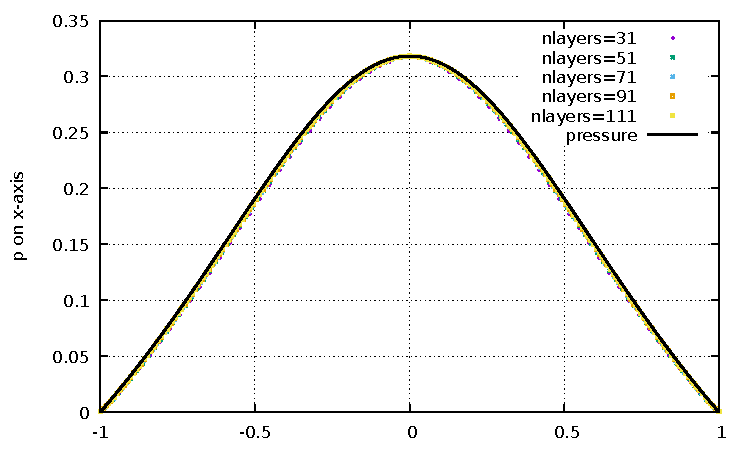
\includegraphics[width=7.3cm]{python_codes/fieldstone_58/experiment1/press_xaxis.pdf}
b)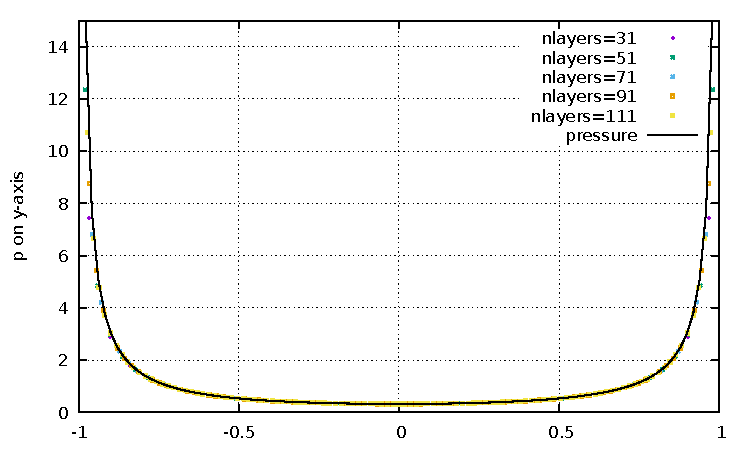
\includegraphics[width=7.3cm]{python_codes/fieldstone_58/experiment1/press_yaxis.pdf}\\
c)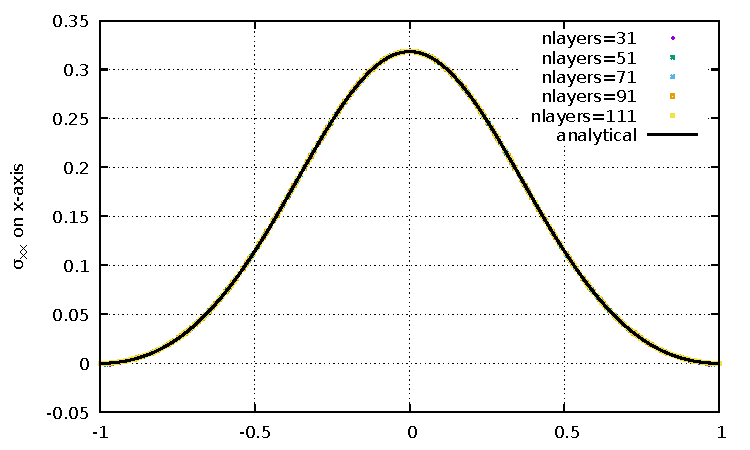
\includegraphics[width=7.3cm]{python_codes/fieldstone_58/experiment1/sigmaxx_xaxis.pdf}
d)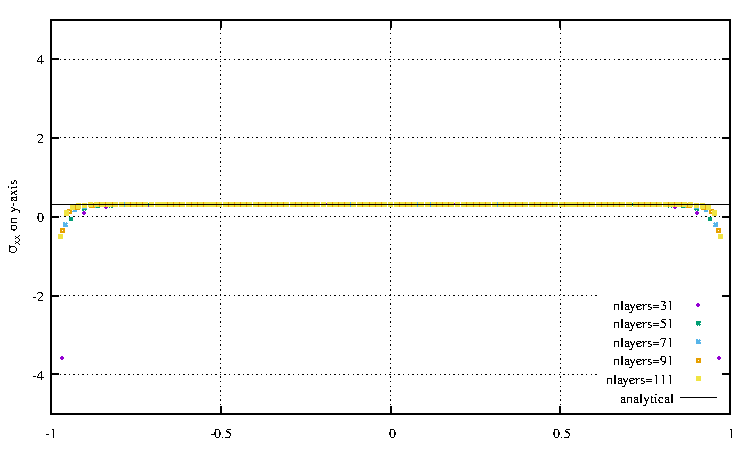
\includegraphics[width=7.3cm]{python_codes/fieldstone_58/experiment1/sigmaxx_yaxis.pdf}\\
e)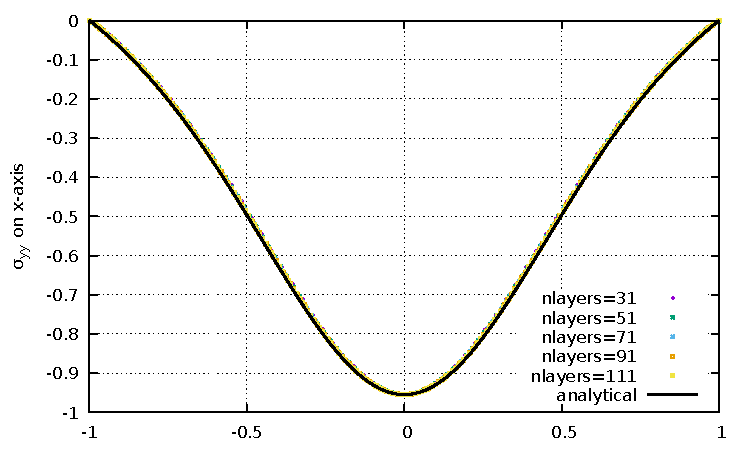
\includegraphics[width=7.3cm]{python_codes/fieldstone_58/experiment1/sigmayy_xaxis.pdf}
f)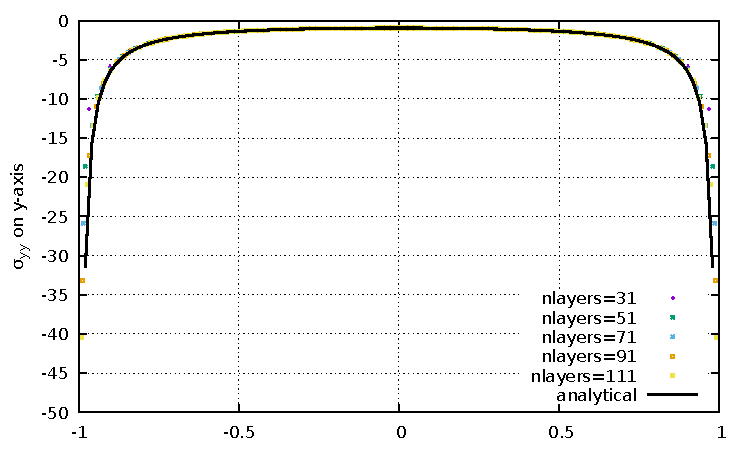
\includegraphics[width=7.3cm]{python_codes/fieldstone_58/experiment1/sigmayy_yaxis.pdf}\\
g)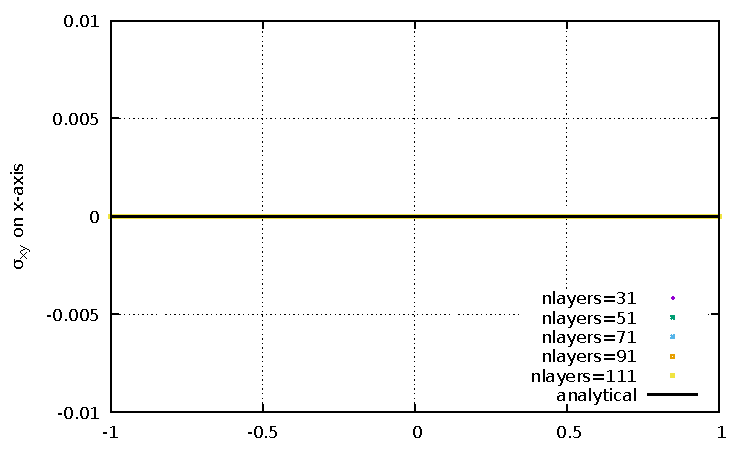
\includegraphics[width=7.3cm]{python_codes/fieldstone_58/experiment1/sigmaxy_xaxis.pdf}
h)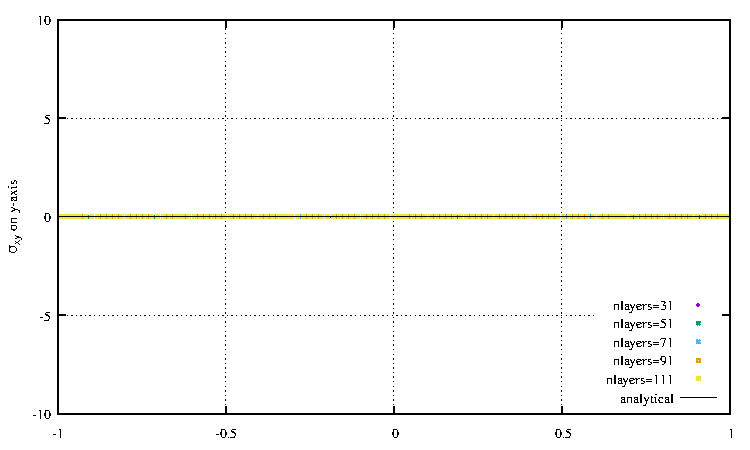
\includegraphics[width=7.3cm]{python_codes/fieldstone_58/experiment1/sigmaxy_yaxis.pdf}\\
i)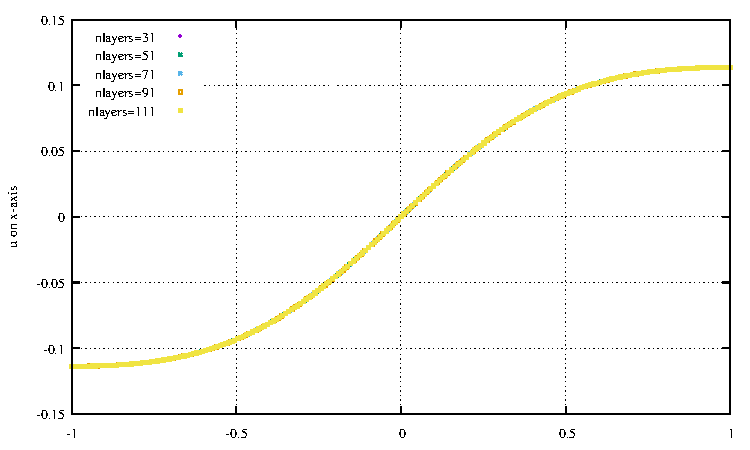
\includegraphics[width=7.3cm]{python_codes/fieldstone_58/experiment1/u_xaxis.pdf}
j)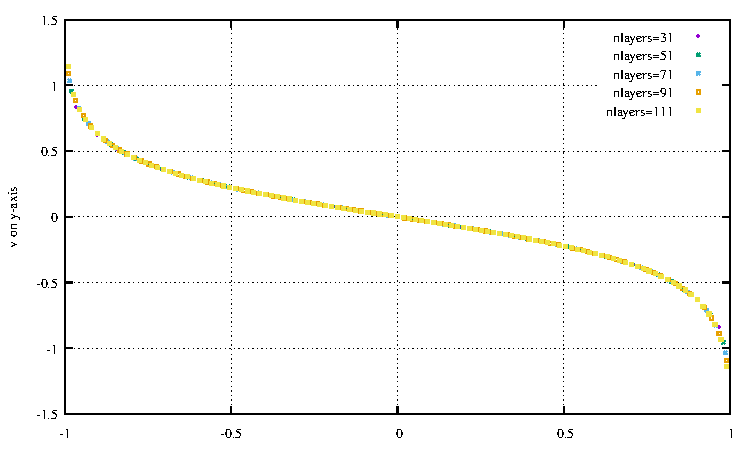
\includegraphics[width=7.3cm]{python_codes/fieldstone_58/experiment1/v_yaxis.pdf}\\
{\captionfont a,b) pressure along the $x$-axis;
c,d) $\sigma_{xx}$  along the $x-$ and $y-$axis; 
e,f) $\sigma_{yy}$  along the $x-$ and $y-$axis; 
g,h) $\sigma_{xy}$  along the $x-$ and $y-$axis; 
i) horizontal displacement along the $x-$axis; 
j) vertical displacement along the $y-$axis}
\end{center}

\newpage
\begin{center}
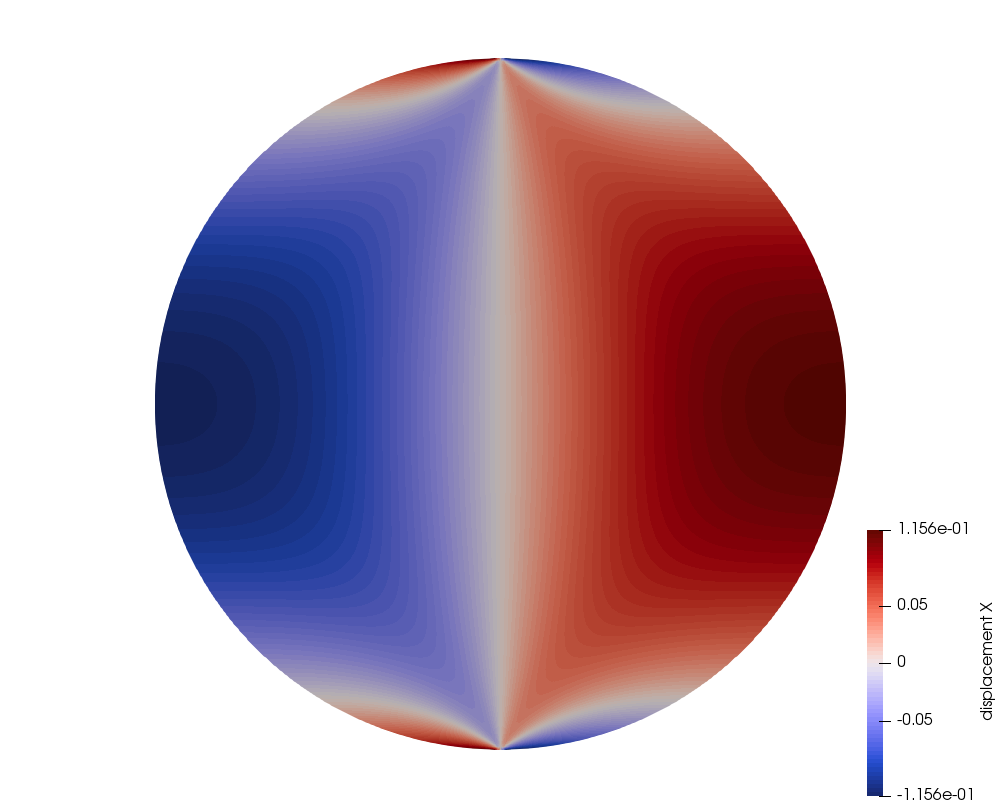
\includegraphics[width=5.4cm]{python_codes/fieldstone_58/experiment1/111/u}
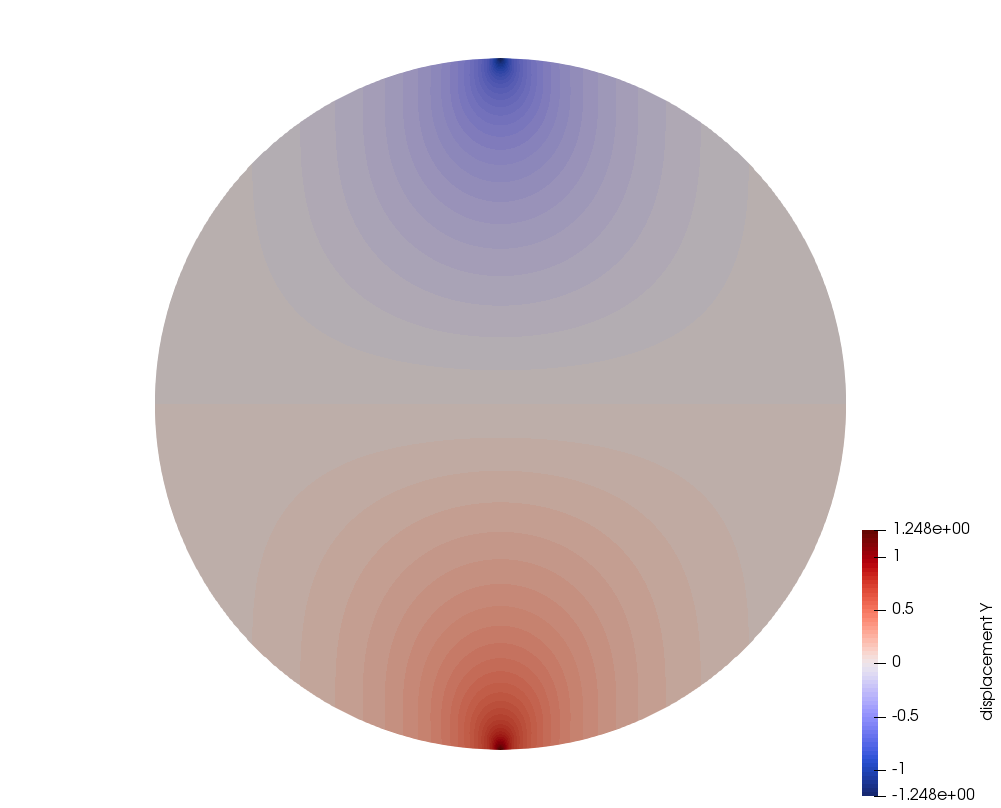
\includegraphics[width=5.4cm]{python_codes/fieldstone_58/experiment1/111/v}
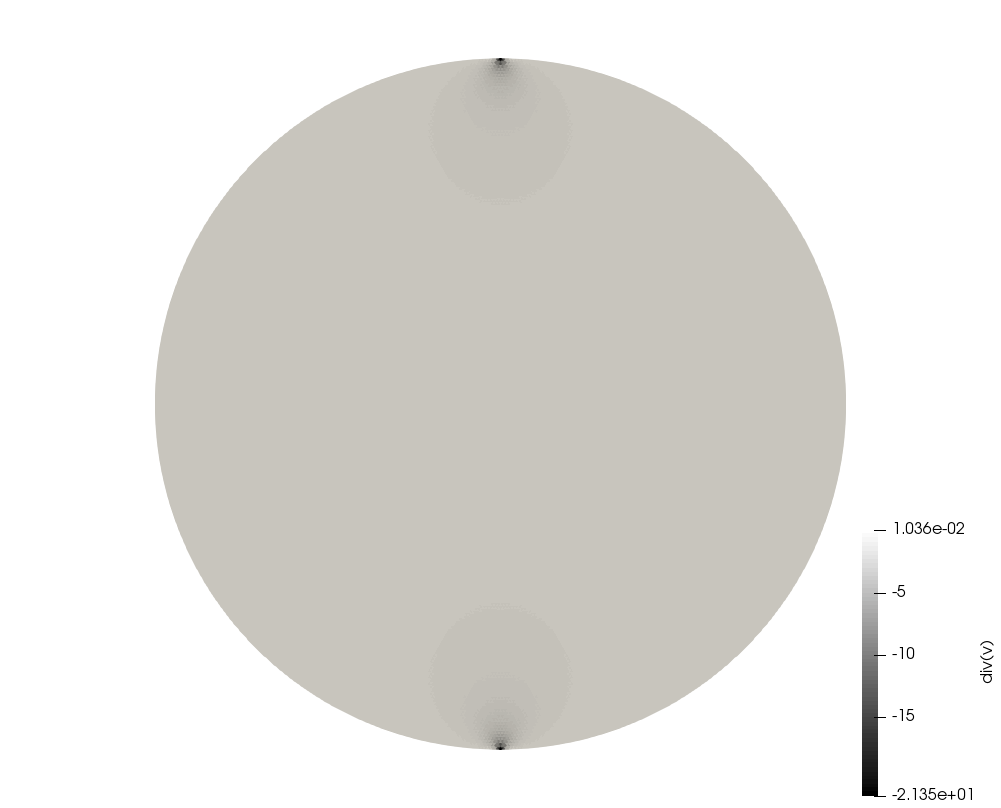
\includegraphics[width=5.4cm]{python_codes/fieldstone_58/experiment1/111/divv}\\
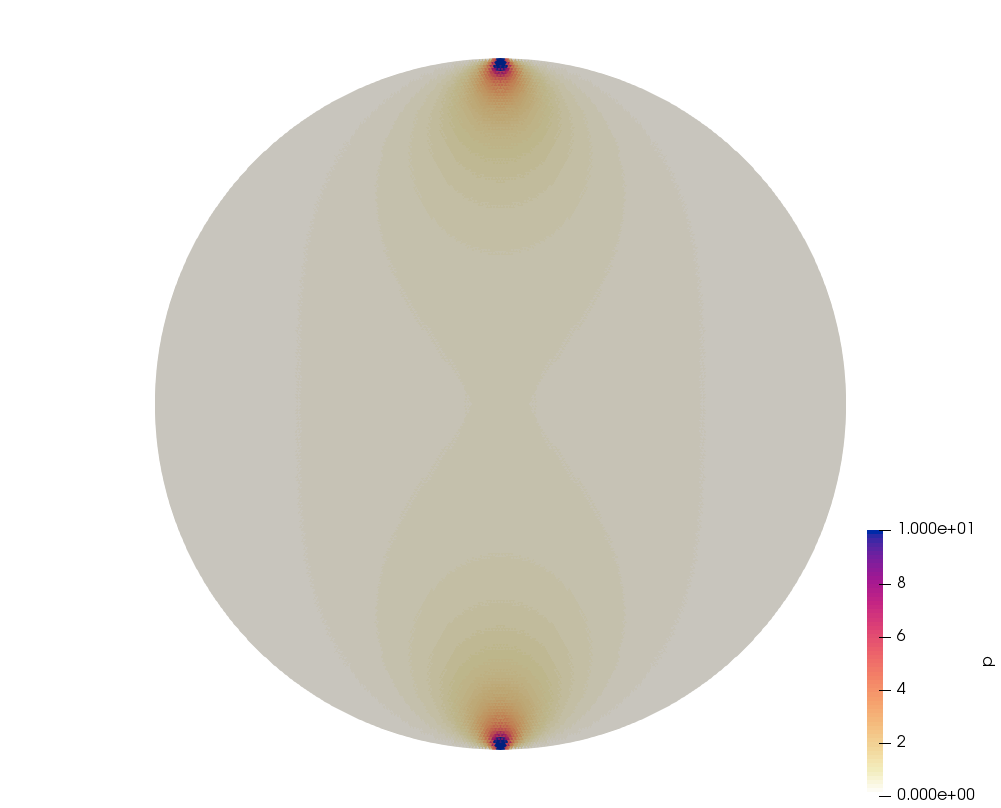
\includegraphics[width=5.4cm]{python_codes/fieldstone_58/experiment1/111/p}
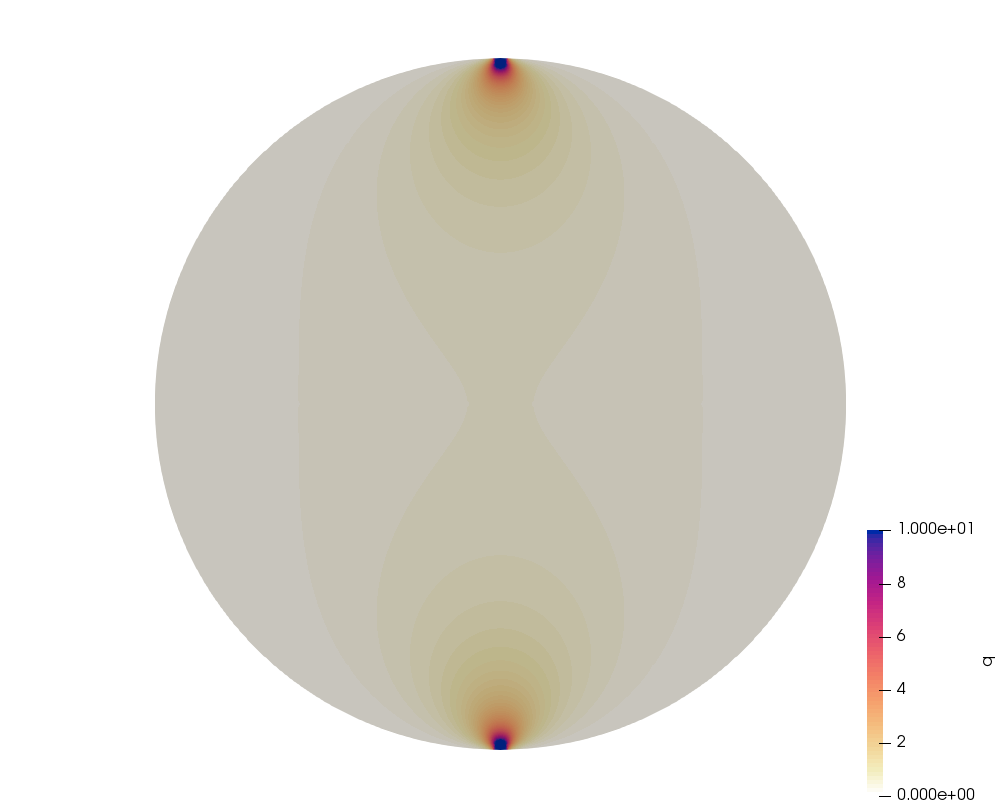
\includegraphics[width=5.4cm]{python_codes/fieldstone_58/experiment1/111/q}
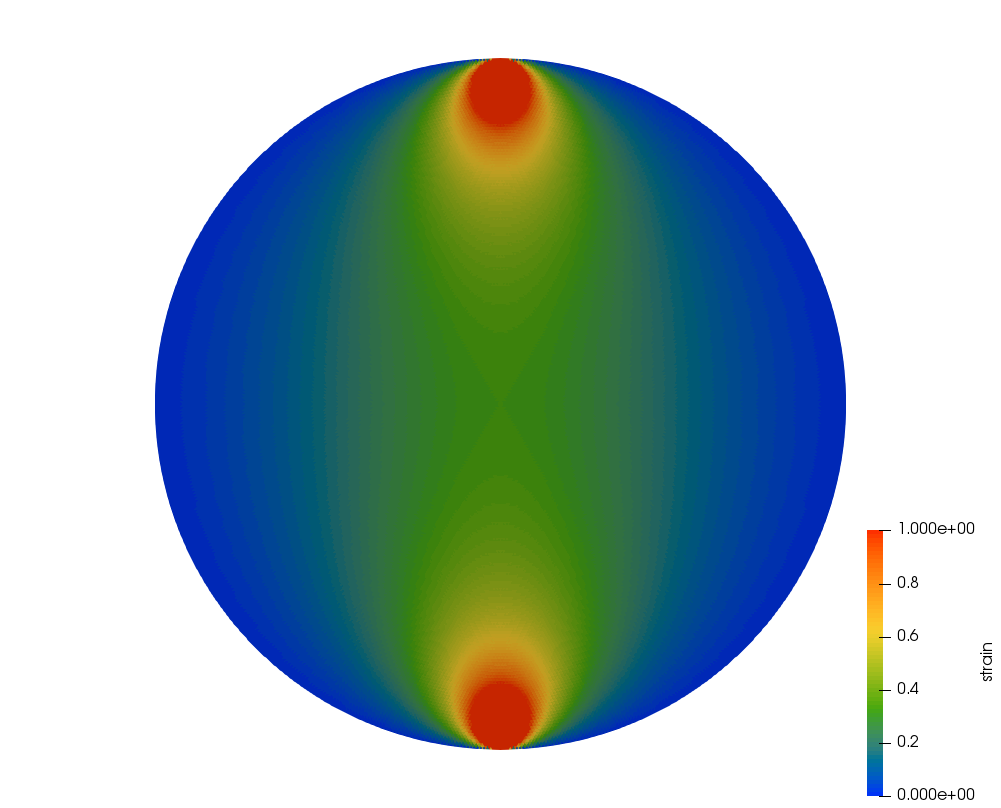
\includegraphics[width=5.4cm]{python_codes/fieldstone_58/experiment1/111/e}\\
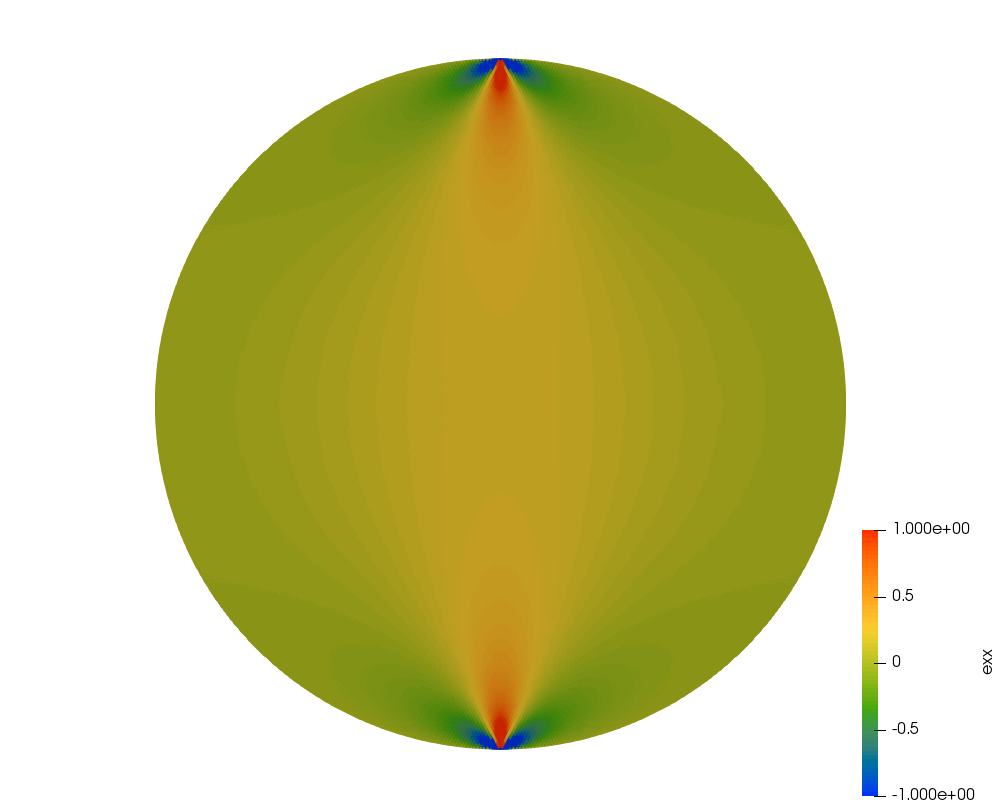
\includegraphics[width=5.4cm]{python_codes/fieldstone_58/experiment1/111/exx}
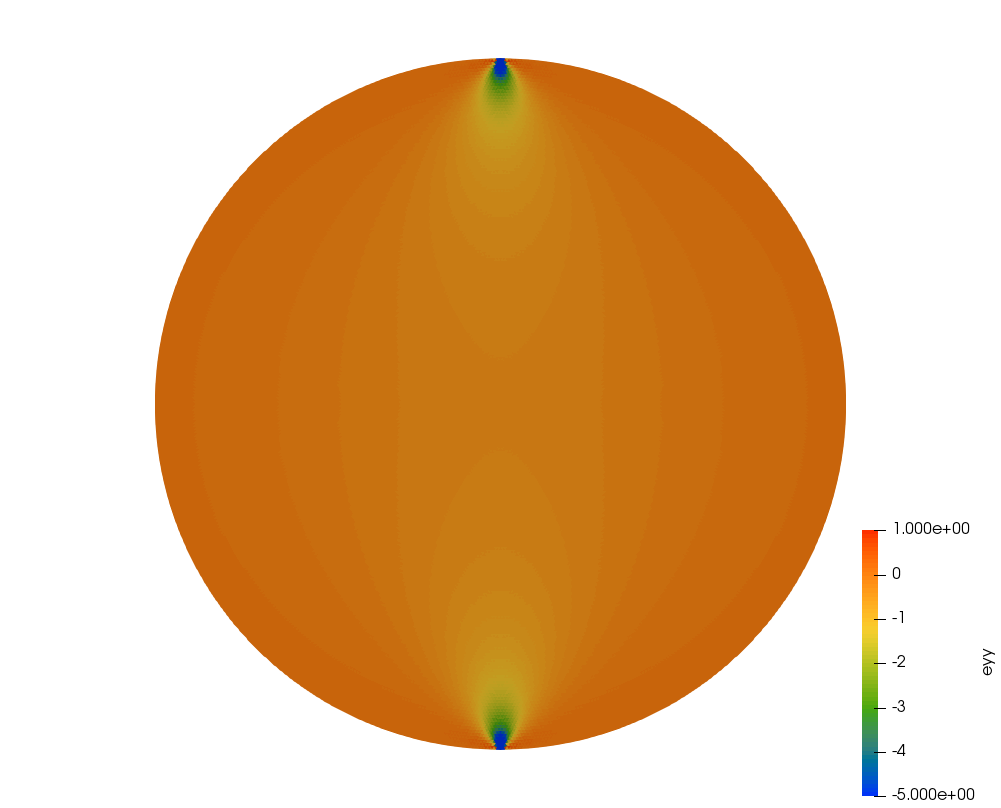
\includegraphics[width=5.4cm]{python_codes/fieldstone_58/experiment1/111/eyy}
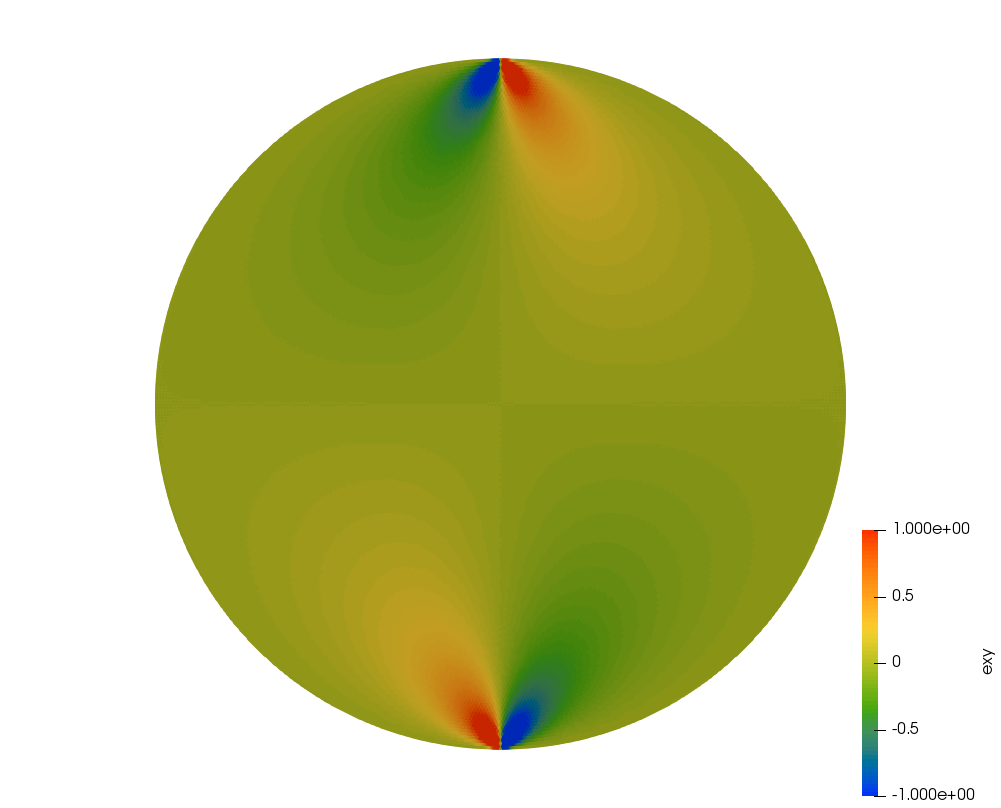
\includegraphics[width=5.4cm]{python_codes/fieldstone_58/experiment1/111/exy}\\
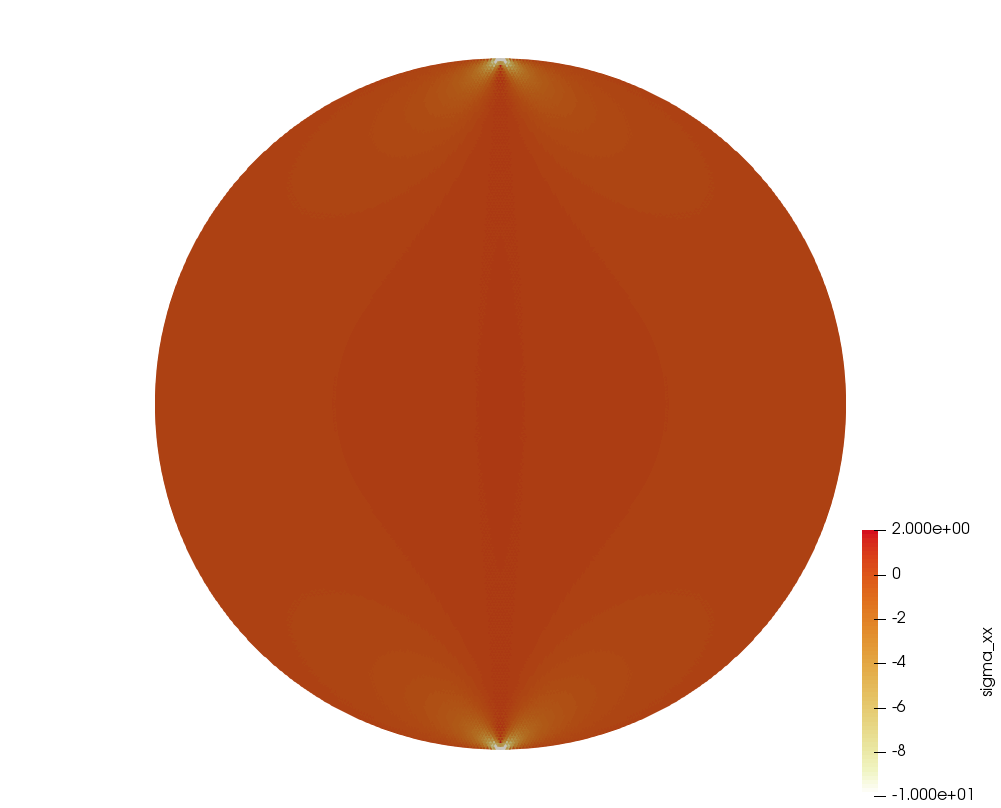
\includegraphics[width=5.4cm]{python_codes/fieldstone_58/experiment1/111/sigma_xx}
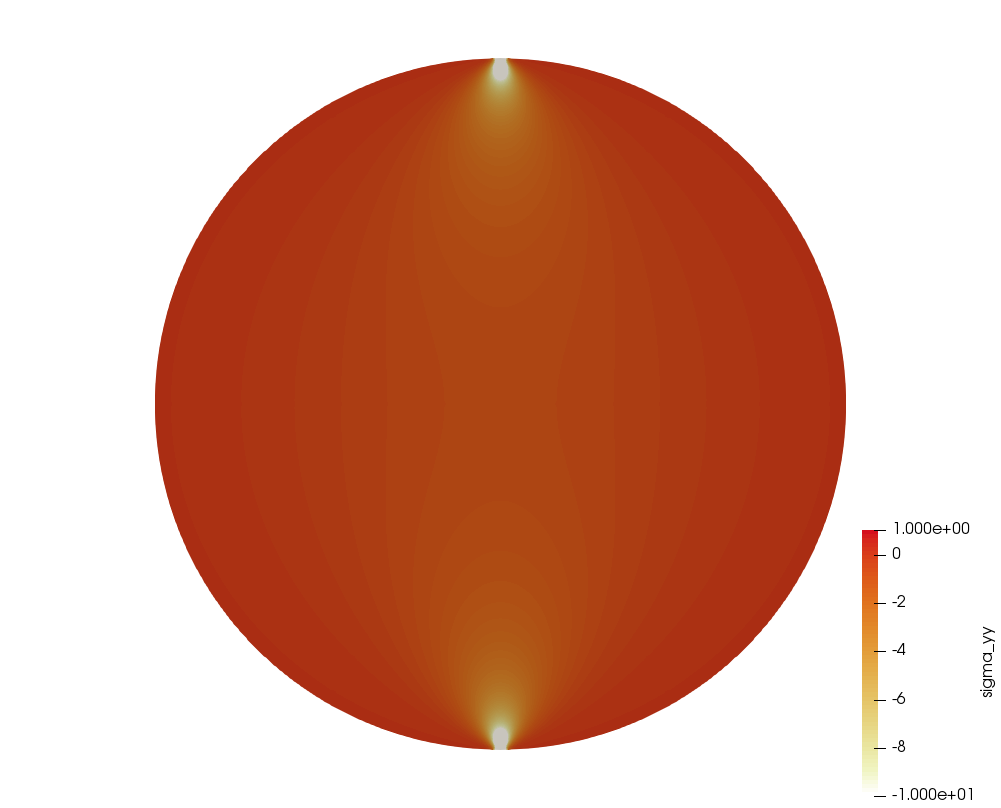
\includegraphics[width=5.4cm]{python_codes/fieldstone_58/experiment1/111/sigma_yy}
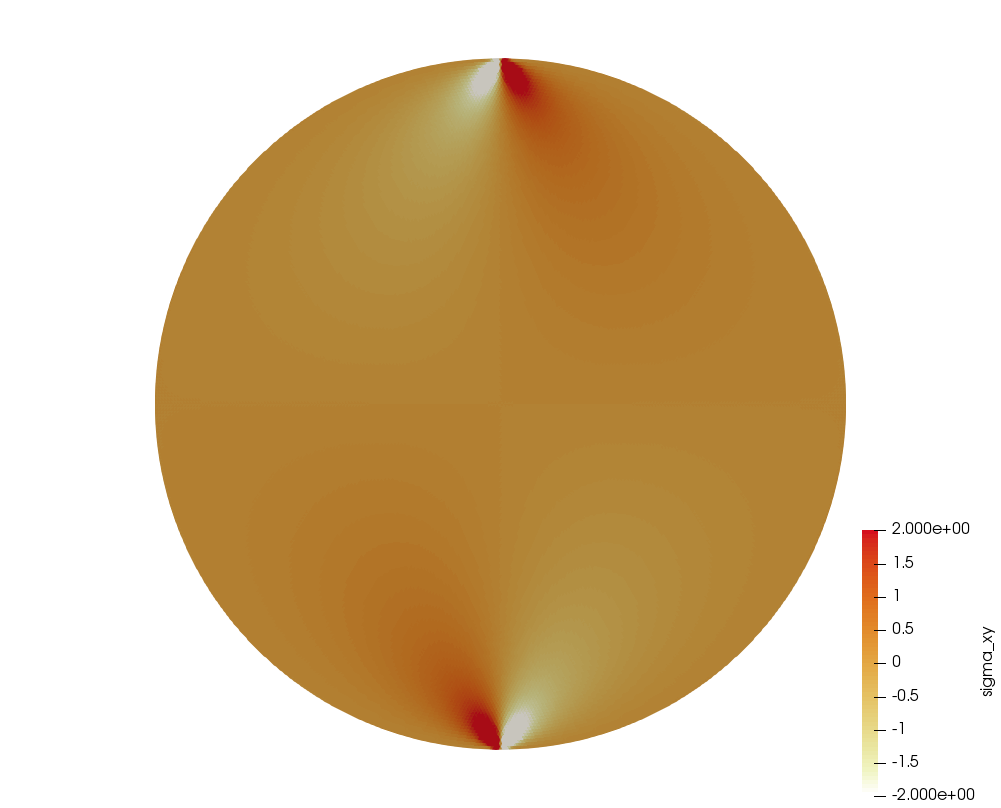
\includegraphics[width=5.4cm]{python_codes/fieldstone_58/experiment1/111/sigma_xy}\\
{\captionfont Results for nLayers=11}
\end{center}

\newpage

\begin{center}
a)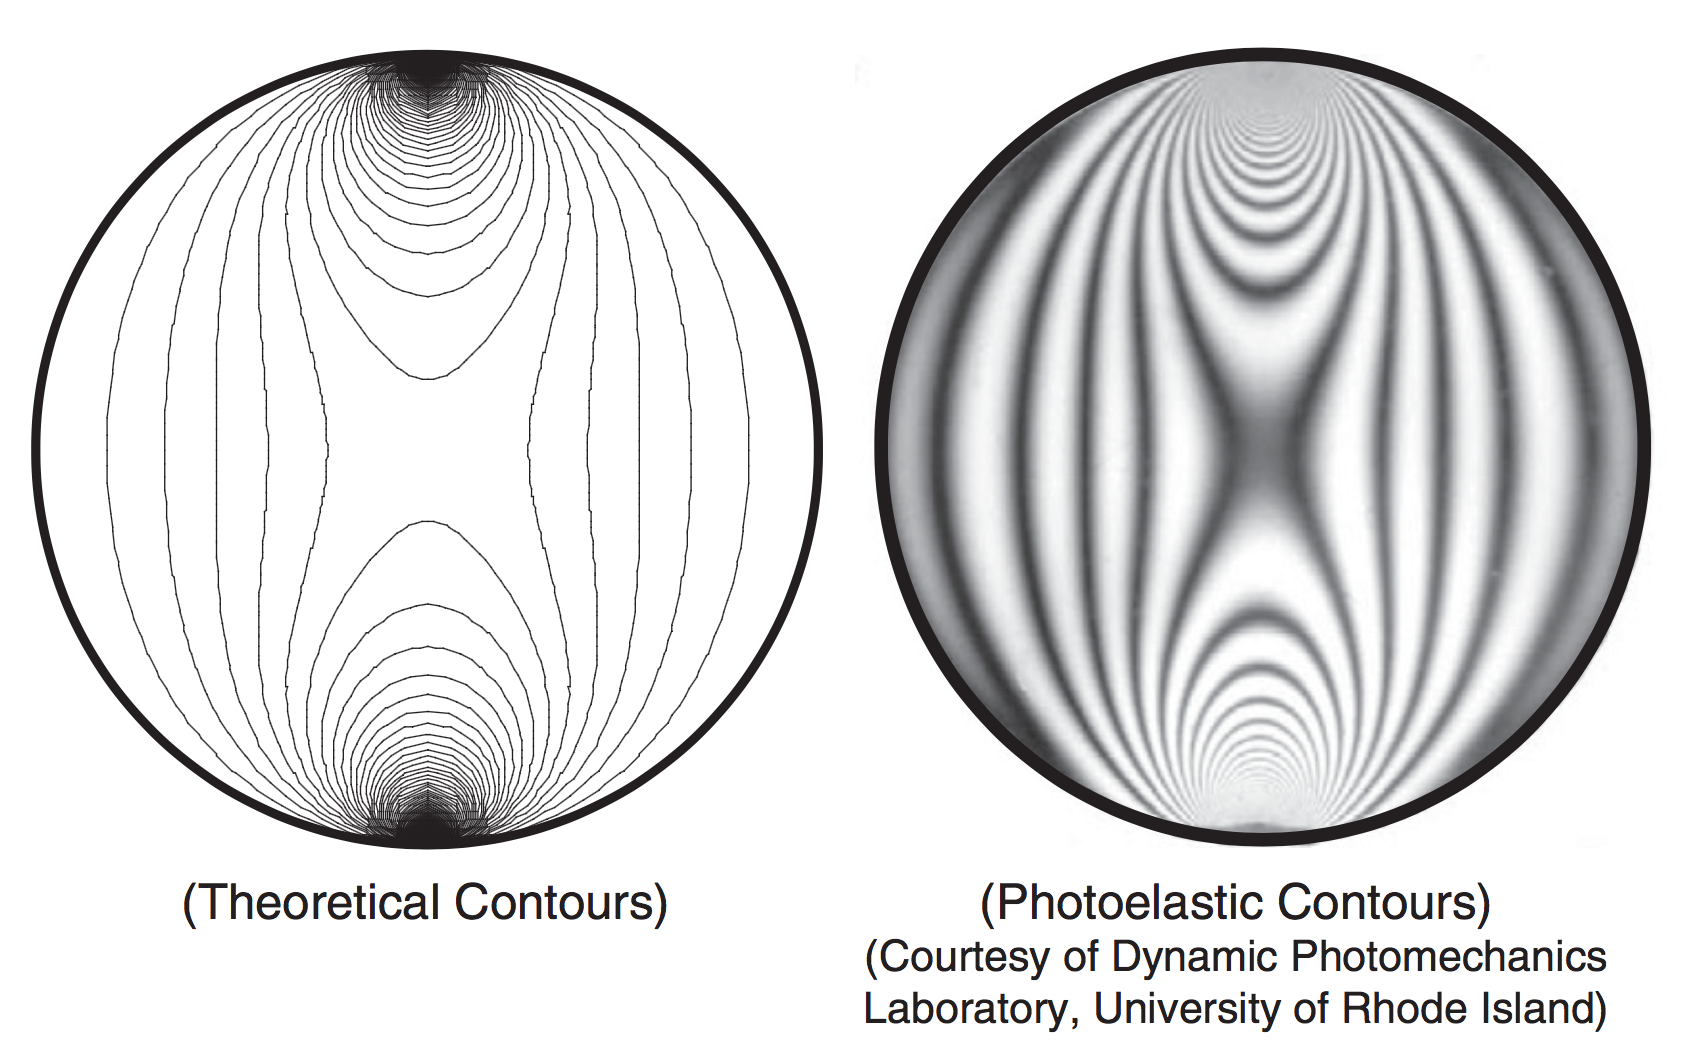
\includegraphics[width=8cm]{python_codes/fieldstone_58/experiment1/contours}
b)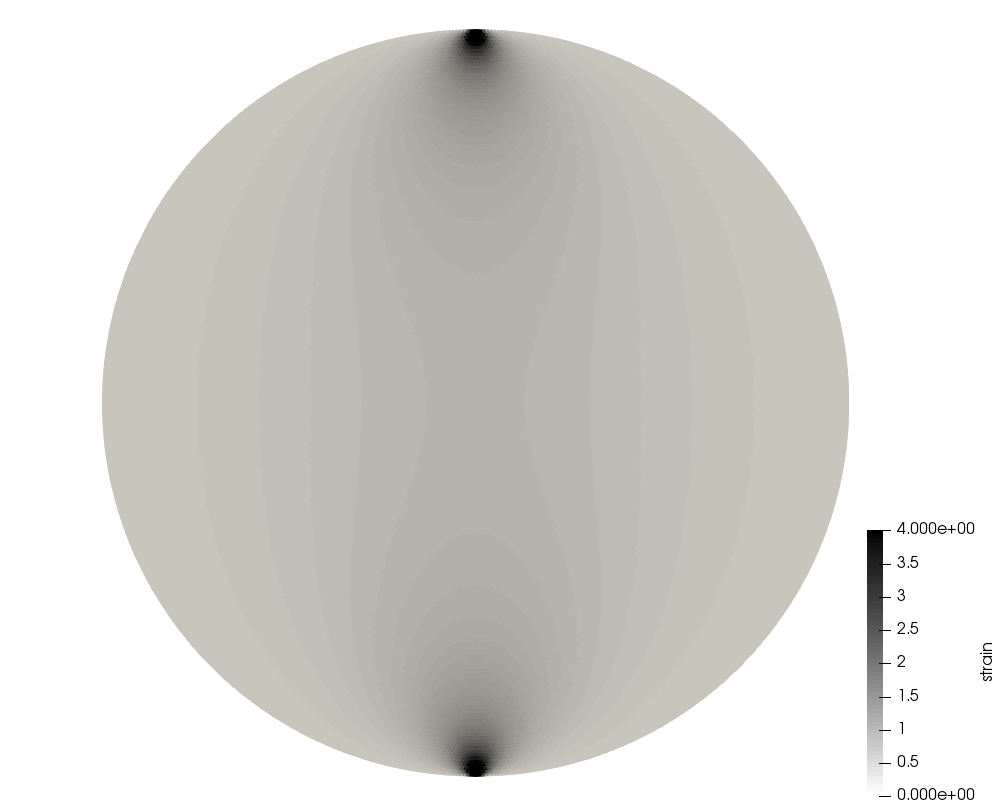
\includegraphics[width=5cm]{python_codes/fieldstone_58/experiment1/111/e_2}\\
{\captionfont 
a) Maximum shear stress contours and corresponding photoelastic isochromatic 
for a disk under diametrical compression \cite{sadd14};\\
b) computed second invariant of the strain tensor.}
\end{center}


We can also look at the principal stresses.
The principal direction angle $\theta_p$ defines the principal
directions where the only stresses are normal stresses, and 
is given by the relationship:
\[
\tan (2\theta_p) =  \frac{2 \sigma_{xy}}{\sigma_{xx} -\sigma_{yy}}
\]
The principal stresses are found from the original stresses via
 \[
\sigma_{1,2}=\frac{\sigma_{xx}+\sigma_{yy}}{2} \pm \sqrt{  \left(\frac{\sigma_{xx}-\sigma_{yy}}{2}\right)^2 +\sigma_{xy}^2 }
 \]



\newpage
%----------------------------
\subsubsection*{Experiment 2}

This experiment was designed in collaboration with T. Shinohara \index{contributors}{T. Shinohara}. 
Unlike the previous one it does not have an analytical solution. Ideally we wished to look at a 
cluster of grains as shown hereunder. However, because of the symmetries of the problem we can 
here again only model one grain, with (idealised) boundary conditions:
 
\begin{center}
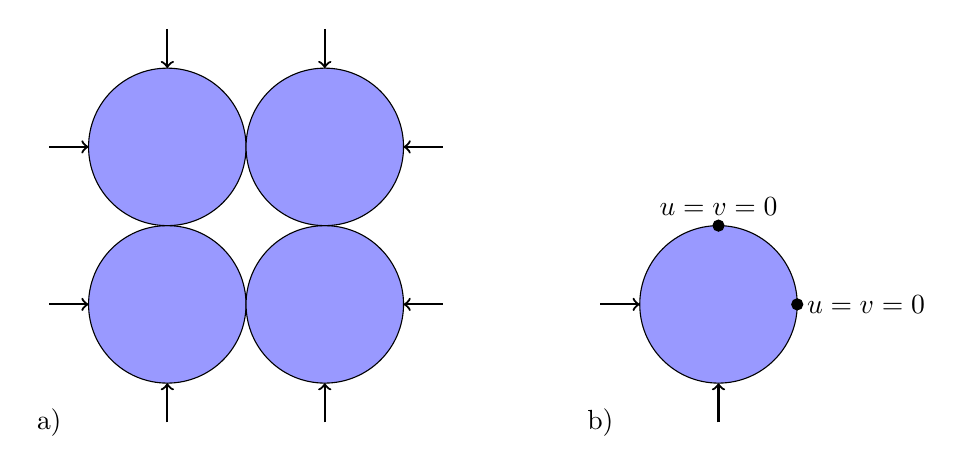
\begin{tikzpicture}
%\draw[fill=gray!23,gray!23](0,0) rectangle (11,6);
%\draw[step=0.5cm,gray,very thin] (0,0) grid (11,6); %background grid
\filldraw[fill=blue!40!white, draw=black] (2,2) circle (1cm);
\filldraw[fill=blue!40!white, draw=black] (4,2) circle (1cm);
\filldraw[fill=blue!40!white, draw=black] (2,4) circle (1cm);
\filldraw[fill=blue!40!white, draw=black] (4,4) circle (1cm);
\draw[thick,->] (0.5,2) -- (1,2); \draw[thick,->] (5.5,2) -- (5,2);
\draw[thick,->] (0.5,4) -- (1,4); \draw[thick,->] (5.5,4) -- (5,4);
\draw[thick,->] (2,0.5) -- (2,1); \draw[thick,->] (2,5.5) -- (2,5);
\draw[thick,->] (4,0.5) -- (4,1); \draw[thick,->] (4,5.5) -- (4,5);
\draw[thick,->] (7.5,2) -- (8,2);
\draw[thick,->] (9,0.5) -- (9,1); 
\filldraw[fill=blue!40!white, draw=black] (9,2) circle (1cm);
\filldraw[black] (10,2) circle (2pt) node[anchor=west] {$u=v=0$};
\filldraw[black] (9,3) circle (2pt) node[anchor=south] {$u=v=0$};
\node[] at (0.5,0.5)   {a)};
\node[] at (7.5,0.5)   {b)};
\end{tikzpicture}\\
{\captionfont a) assembly of four circular grains and the pressure boundary conditions; 
b) simplified setup of a single grain.}
\end{center}

\begin{center}
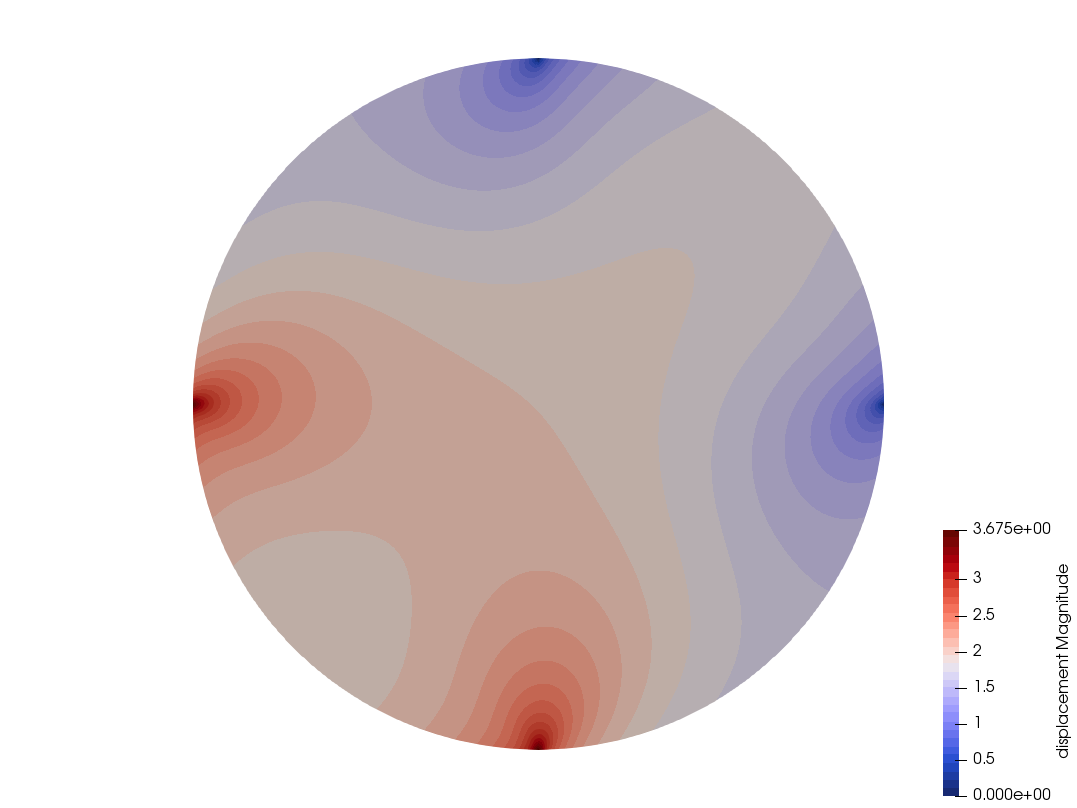
\includegraphics[width=5.5cm]{python_codes/fieldstone_58/experiment2/displ}
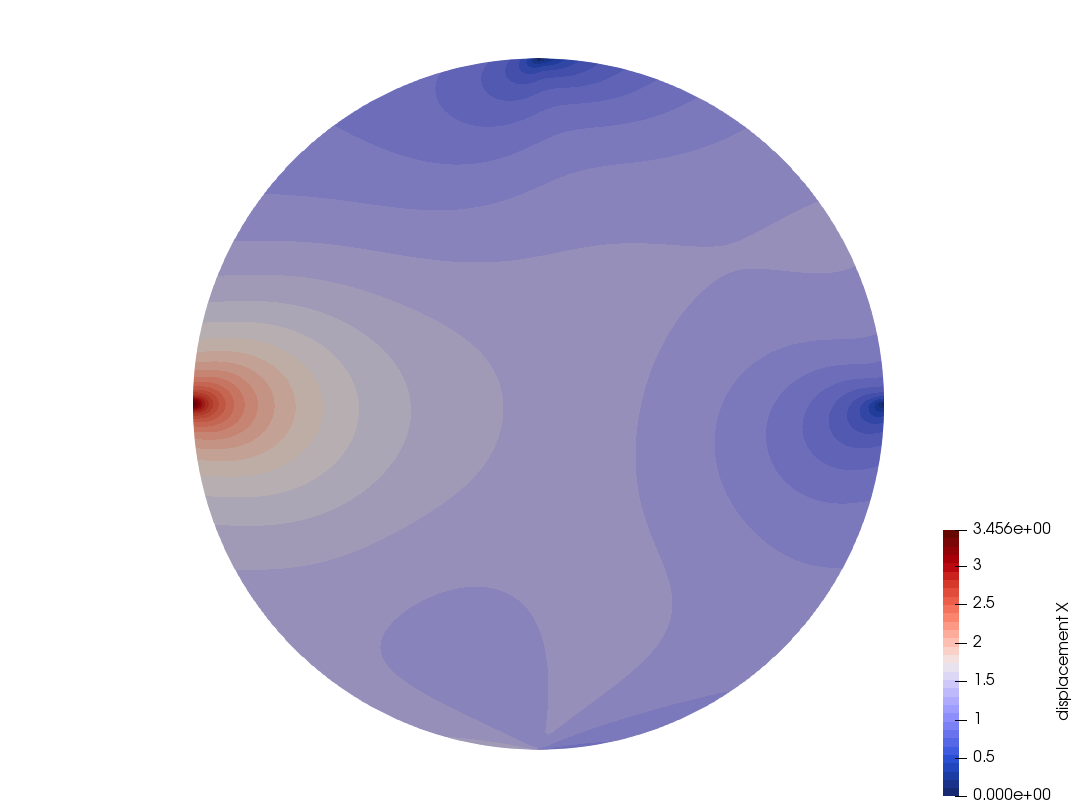
\includegraphics[width=5.5cm]{python_codes/fieldstone_58/experiment2/displx}
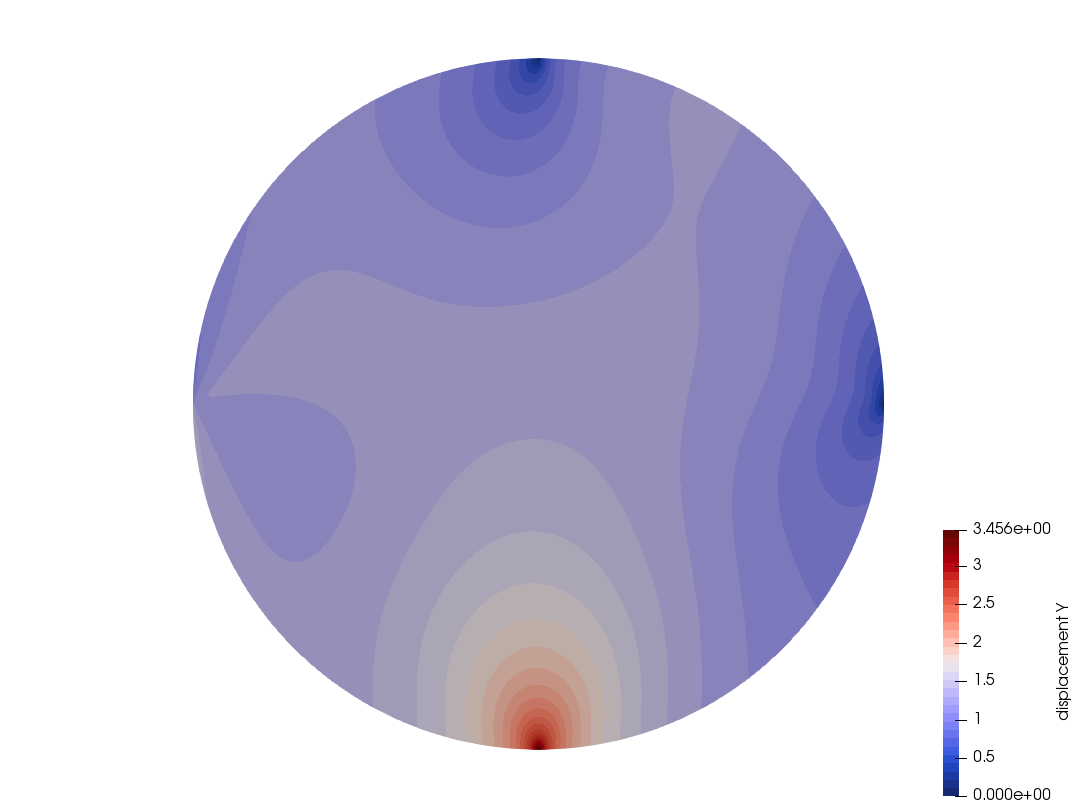
\includegraphics[width=5.5cm]{python_codes/fieldstone_58/experiment2/disply}\\
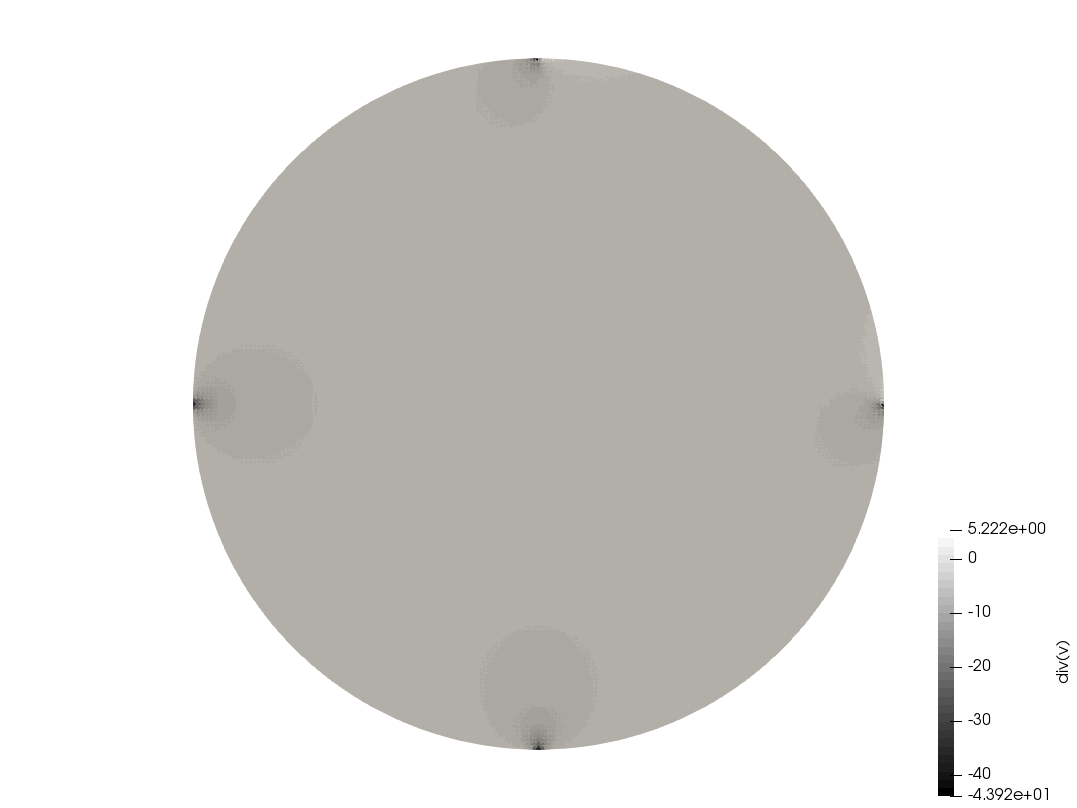
\includegraphics[width=5.5cm]{python_codes/fieldstone_58/experiment2/divv}
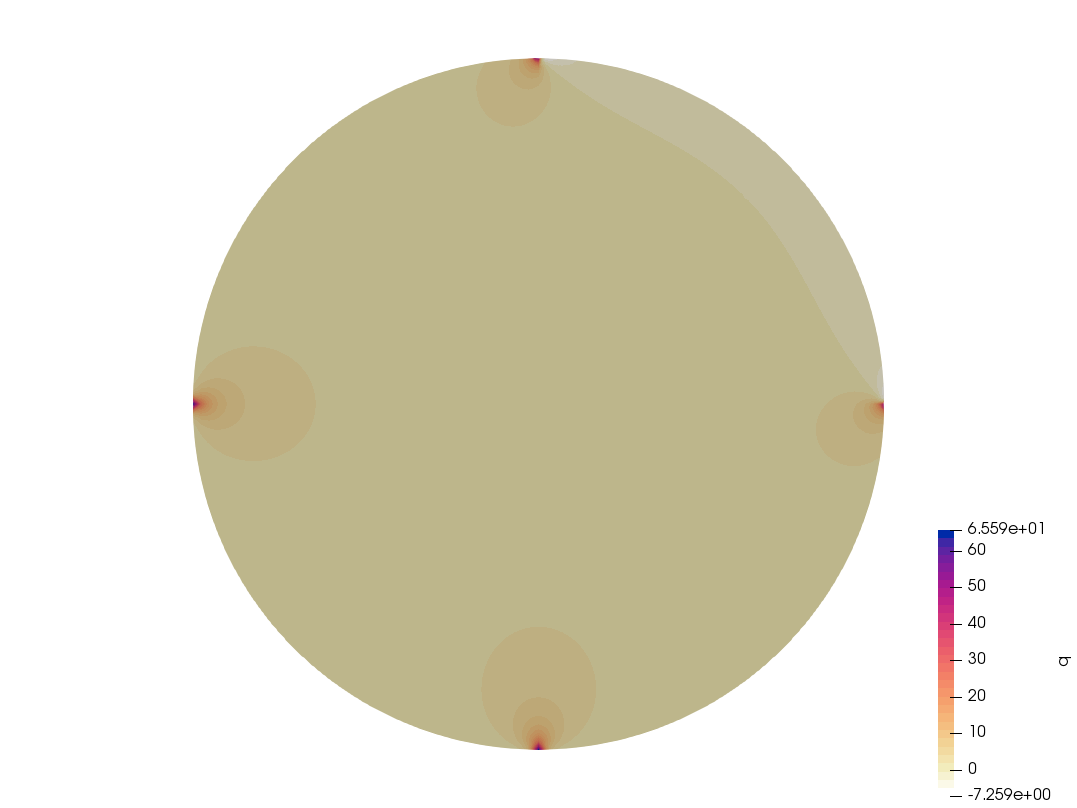
\includegraphics[width=5.5cm]{python_codes/fieldstone_58/experiment2/p}
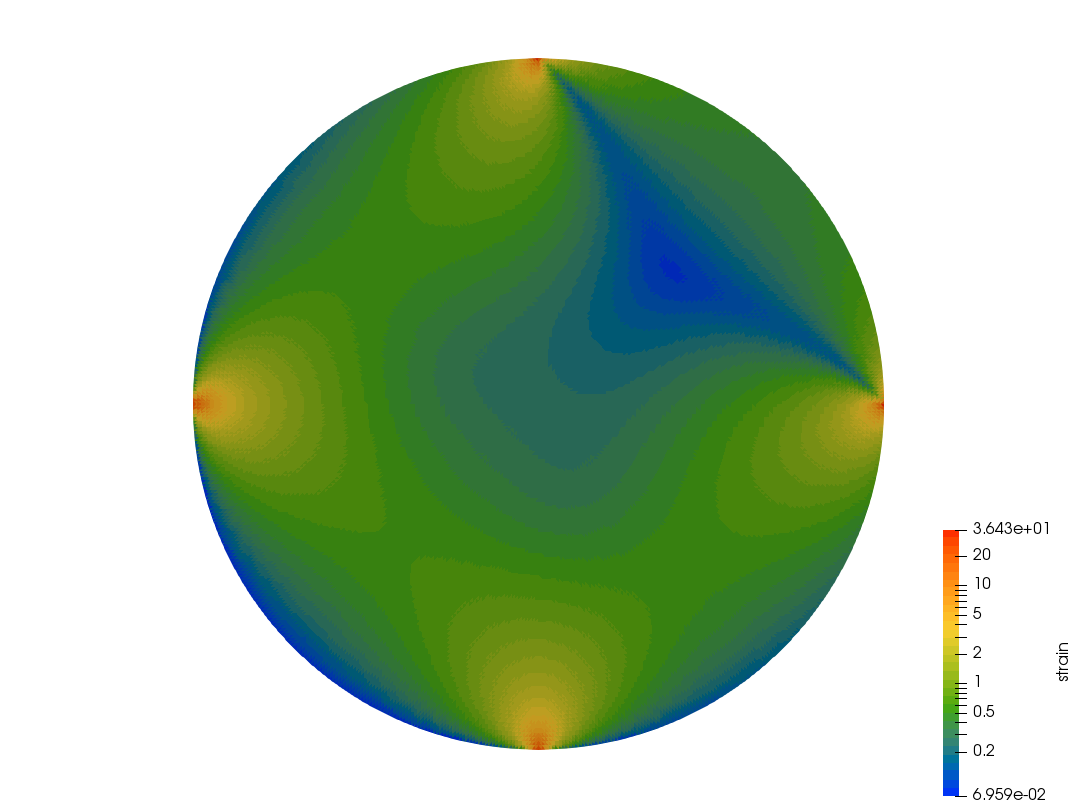
\includegraphics[width=5.5cm]{python_codes/fieldstone_58/experiment2/strain}\\
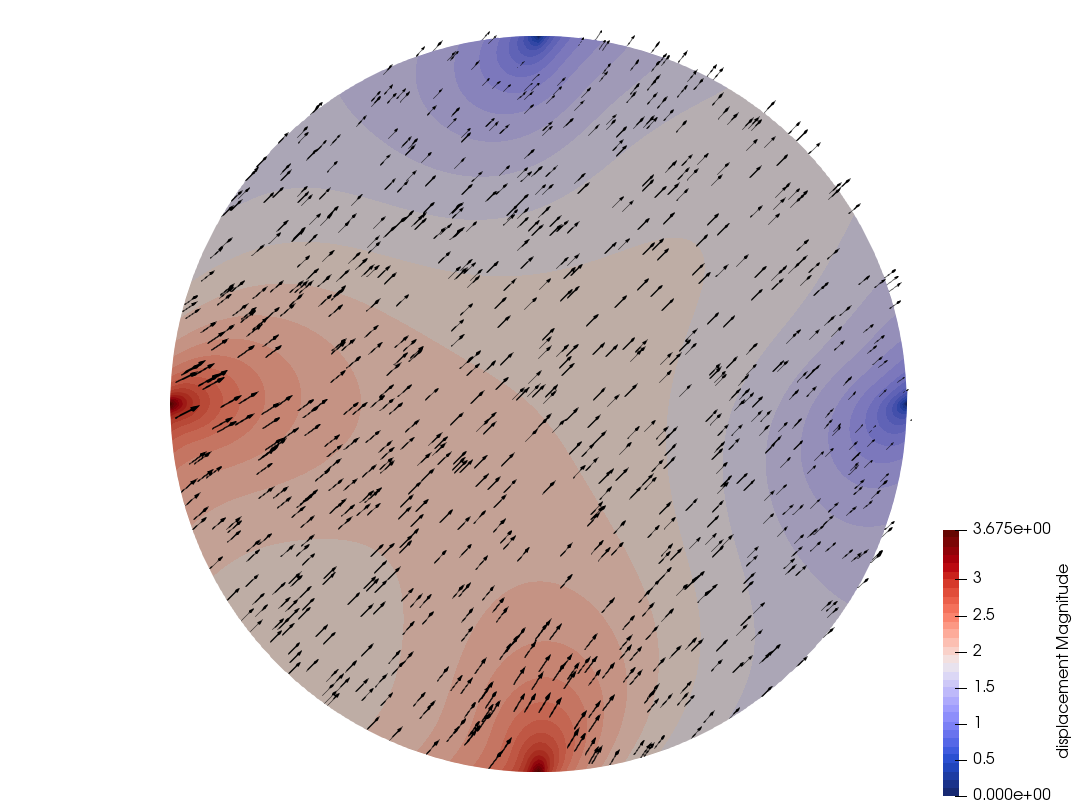
\includegraphics[width=10cm]{python_codes/fieldstone_58/experiment2/dispvect}
\end{center}






